\documentclass[a4paper,DIV11,bibliography=totoc,headings=normal,ngerman,headsepline]{scrreprt}

%Benötigte Packages
\usepackage{babel} 
\usepackage[T1]{fontenc}           
\usepackage[utf8]{inputenc}  
\usepackage{graphicx}
\usepackage{amsmath}

%Literaturverzeichnis
\usepackage[backend=biber]{biblatex}
\usepackage[babel,german=quotes]{csquotes}

%Formelverzeichnis mittels KOMA-Script erstellen
\DeclareNewTOC[type=formel,name={Formel},hang=5em,listname={Formelverzeichnis}]{for}
\newcommand*{\formelentry}[1]{\addcontentsline{for}{formel}{\protect\numberline{Formel~\theequation} #1}}

%Informationen der PDF
\pdfinfo
{
/Title		(Extrapolation von Zeitreihen mit Hilfe von künstlichen neuronalen Netzen am Beispiel von Börsenprognosen)
/Subject	(Eine Anwendung im Fach Softcomputing – Teilgebiet neuronale Netze)
/Author		(Sebastian Schötteler \& Benedikt Hofrichter)
}

%Kopf- und Fußzeile
\pagestyle{headings}

\begin{document}

\subject{Seminararbeit}
\title{Extrapolation von Zeitreihen mit Hilfe von künstlichen neuronalen Netzen am Beispiel von Börsenprognosen}
\author{Sebastian Schötteler -- Matrikelnummer 2429289 \and Benedikt Hofrichter -- Matrikelnummer 2272198}
\publishers{Technische Hochschule Nürnberg Georg Simon Ohm}

%Zur Überscchrift machen
\maketitle

%Verzeichnisse
\tableofcontents
\listoffigures
\listoftables
\listofformels

\chapter{Einleitung} %Beide
\section{Motivation}
Die Untersuchung  und Extrapolation von Zeitreihen ist ein bedeutendes Thema in zahlreichen Gebieten. Typische Anwendungsbereiche sind dabei Prognose von Wetterdaten, von Therapieverläufen in der  Medizin und Psychologie, von Arbeitslosenzahlen auf dem Arbeitsmarkt sowie Börsenkursen. Um eine Zeitreihe möglichst genau zu extrapolieren, wird auf mehreren Hilfsmitteln zugegriffen. Einer dieser Hilfsmittel sind künstliche neuronale Netze (Abgekürzt: KNN). Bei künstlichen neuronale Netzen handelt es sich um ein in sich geschlossenes System von Neuronen, die die Eingabe weiterverarbeiten und das Ergebnis an weitere Neuronen weiterleiten.  
Die Untersuchung  und Extrapolation von Zeitreihen ist ein bedeutendes Thema in zahlreichen Gebieten. Typische Anwendungsbereiche sind dabei Prognose von Wetterdaten, von Therapieverläufen in der  Medizin und Psychologie, von Arbeitslosenzahlen auf dem Arbeitsmarkt sowie Börsenkursen. Um eine Zeitreihe möglichst genau zu extrapolieren, wird auf mehreren Hilfsmitteln zugegriffen. Einer dieser Hilfsmittel sind künstliche neuronale Netze (Abgekürzt: KNN). Bei künstlichen neuronale Netzen handelt es sich um ein in sich geschlossenes System von Neuronen, die die Eingabe weiterverarbeiten und das Ergebnis an weitere Neuronen weiterleiten. 
Die Untersuchung  und Extrapolation von Zeitreihen ist ein bedeutendes Thema in zahlreichen Gebieten. Typische Anwendungsbereiche sind dabei Prognose von Wetterdaten, von Therapieverläufen in der  Medizin und Psychologie, von Arbeitslosenzahlen auf dem Arbeitsmarkt sowie Börsenkursen. Um eine Zeitreihe möglichst genau zu extrapolieren, wird auf mehreren Hilfsmitteln zugegriffen. Einer dieser Hilfsmittel sind künstliche neuronale Netze (Abgekürzt: KNN). Bei künstlichen neuronale Netzen handelt es sich um ein in sich geschlossenes System von Neuronen, die die Eingabe weiterverarbeiten und das Ergebnis an weitere Neuronen weiterleiten. 
Die Untersuchung  und Extrapolation von Zeitreihen ist ein bedeutendes Thema in zahlreichen Gebieten. Typische Anwendungsbereiche sind dabei Prognose von Wetterdaten, von Therapieverläufen in der  Medizin und Psychologie, von Arbeitslosenzahlen auf dem Arbeitsmarkt sowie Börsenkursen. Um eine Zeitreihe möglichst genau zu extrapolieren, wird auf mehreren Hilfsmitteln zugegriffen. Einer dieser Hilfsmittel sind künstliche neuronale Netze (Abgekürzt: KNN). Bei künstlichen neuronale Netzen handelt es sich um ein in sich geschlossenes System von Neuronen, die die Eingabe weiterverarbeiten und das Ergebnis an weitere Neuronen weiterleiten. 

\section{Ziel dieser Arbeit}
Die Funktionsweise und Effektivität von KNN bei der Extrapolation von Zeitreihen soll anhand einer Anwendung, die den Boersenkurs des DAX für die nächsten Börsentage prognostiziert, ermittelt und anschließend demonstriert werden.
 
\chapter{Konzeption} %Beide
\section{Fachliche Konzeption der Anwendung} %Benedikt
\subsection{Funktionalitäten der Anwendung} %Benedikt
\subsection{Mockup der Anwendung} %Benedikt

\begin{figure}[htbp]
\centering
		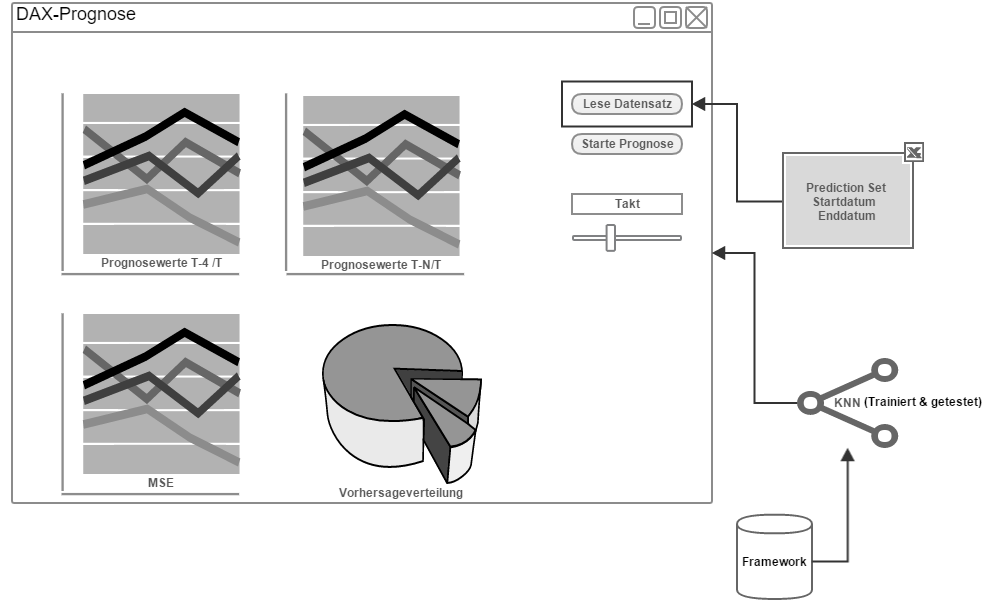
\includegraphics[width=0.80\textwidth]{mockup.PNG}
	\caption{Mockup der Anwendung}
	\label{fig:Mockup der Anwendung}
\end{figure}


\section{Konzeption des künstlichen neuronalen Netzes} %Sebastian
\subsection{Typ des künstlichen neuronalen Netzes} %Sebastian
\subsection{Architektur des künstlichen neuronalen Netzes} %Sebastian
\subsection{Lernverfahren des künstlichen neuronalen Netzes} %Sebastian
\section{Beschreibung von Frameworks} %Benedikt
\subsection{SNNS} %Benedikt
\subsection{JavaNNS}  %Benedikt
\subsection{Neuroph} %Benedikt
\section{Wahl des geeignetsten Frameworks} %Benedikt
\chapter{Umsetzung} %Beide
\section{Erstellung des künstlichen neuronalen Netzes} %Sebastian

\subsection{Wahl der Topologie} %Sebastian
In der Literatur wird dabei oft auf die folgende Gleichung zur Ermittlung der optimalen  Menge an Neuronen der versteckten Schicht angegeben:

\begin{equation}\formelentry{Optimale Anzahl Neuronen in der versteckten Schicht}
  N_h = \frac{N_d}{10*(N_i+N_o)}
\end{equation}

\subsection{Wahl der Transferfunktion} %Sebastian

Sigmoide Funktion:

\begin{equation}\formelentry{Sigmoide Funktion}
f(x)= \frac{1}{1+e^{-cx}}
\end{equation}

Tangens Hyperbolicus:

\begin{equation}\formelentry{Tanh Funktion}
f(x)= tanh(x)
\end{equation}

\subsection{Wahl der Lernregel} %Sebastian
\section{Überführung des künstlichen neuronalen Netzes in einer Anwendung}
\section{Umsetzen der Anwendung} %Benedikt

\chapter{Beschreibung der Anwendung} %Benedikt
\section{Elemente der GUI} %Beide
\section{Architektur der Anwendung} %Benedikt
\section{Zusammenspiel mit dem Framework} %Sebastian

\chapter{Fazit} %Beide
Das prognfsdfdsostizieren von Börsenkursen mittels künstlichen neuronalen Netzen ist möglich.


%%Literaturverzeichnis
%\begin{thebibliography}{999}
%\bibitem{00} Uwe Lämmel \& Jürgen Cleve,\emph{Künstliche Intelligenz}, Hanser Verlag, München, 3., neu bearbeitete Auflage, 2008.
%\end{thebibliography}

%\printbibliography

\end{document}